\chapter{The Learning Algorithm}
\label{chap:Algorithm}

This chapter focuses on the discussion of the deep learning algorithm that has been implemented and tested throughout
the work. Though I have been using such algorithm to perform data quality monitoring tasks, it originates from the
search for new physics at LHC. That being said, in the first part of this chapter I will present the reasons for which
this algorithm has been created, followed by some conceptual foundations and the actual algorithm detailed
description. In the second part of this chapter, the algorithm will be tested using simulated data distributions and its
behavior, performance and results will be discussed. The application of the algorithm to data quality monitoring and
its results can be found in \autoref{chap:Results}.


\section{Introduction to Deep Learning techniques in Physics}
\label{sec:dltphysics}

As more and more data are collected, the problems that physicists are facing become sharper and harder to solve: it is
well known that the currently accepted theories that well describe data (e.g. the Standard Model of particle physics or
the cosmological model $\Lambda$CDM) are incomplete and should be extended. However, the scientific community's prior
beliefs on how such extension should look like keep becoming less concordant. Let us consider the problem of having
large datasets that seem to be well described by the reference model. The main goal is to determine whether the
experimental dataset does follow the reference model exactly or it contains departures as described above. However, the
true underlying data distribution, possibly including new physics effects, will be almost identical to the reference
one: the vast majority of the data collected will agree with the reference model. The most widely employed approach to
the problem is to search for events of specific new physics models. In any such model, one can identify a priori the
subset of data where large departures from the reference model should be concentrated. In this sense, this is a biased
search for anomalies. While this procedure provides a clear physical insight into the new phenomena, scientists have come
to realize that employing a model-dependent approach has a critical disadvantage: a statistical test designed to be
sensitive to one specific hypothesis is typically insensitive to data departures of a different nature from the one
expected. This means that if new physics is present in the data, but not predicted by the specific model that is being
tested, it would not be discovered. 

\subsection{Model-independent approach}

Many attempts at generalizing traditional model-dependent approach have already been made, developing the so-called
model-independent search strategies. It is crucial to remark that model-independent hypothesis testing is an ill-defined
concept in statistics: testing the reference unavoidably requires an alternative hypothesis against which the test is
performed. In a model-independent approach, the alternative hypothesis is not built from a specific physical model but
is a flexible one. The alternative hypothesis is thus a model which specifies a flexible expected density distribution
that can approximate the true underlying data distribution. The algorithm presented in this chapter, proposed in
\cite{zanetti} and \cite{wulzer}, uses NNs to parametrize the alternative distribution to detect deviations from the
reference model in experimental datasets with no prior knowledge of the nature of the discrepancies. 


\section{Conceptual foundations}
\label{sec:foundations}

The whole construction of the statistical foundations that underpin the algorithm is accurately discussed in
\cite{wulzer}, in which only the $1\text{D}$ input dataset scenario is being treated. Although I will not show in this
thesis any practical example or application of the multi-dimensional generalization of the algorithm, in this section I
will recap the main steps of the construction of hypothesis testing without the mono-dimensional constraint, as proposed
in \cite{zanetti}.\\

Let us consider then a dataset of repeated measurements
$\mathbfcal{D}=\{x_i\}_{i=1\,\ldots\,\mathcal{N}_{\mathbfcal{D}}}$ of a \textit{d}-dimensional random variable $x$. Let
$n(x\,|\,\mathbfcal{R})$ be its expected differential distribution as predicted by the reference model
$\mathbfcal{R}\,(\,\equiv H_0$, i.e. the null hypothesis): it can be written as 

\begin{equation}
    n(x\,|\,\mathbfcal{R}) = \mathcal{N}_{\mathbfcal{R}}^{\text{exp}}\,\,p(x\,|\,\mathbfcal{R})
\end{equation}

\noindent where $p(x\,|\,\mathbfcal{R})$ is the probability density function related to the reference hypothesis and
$\mathcal{N}_{\mathbfcal{R}}^{\text{exp}}$ is the total number of expected events to be found in the experimental
dataset according to $\mathbfcal{R}$, given by 

\begin{equation}
    \mathcal{N}_{\mathbfcal{R}}^{\text{exp}}=\int  n(x\,|\,\mathbfcal{R}) \, \text{d}x
\end{equation}


\noindent If the dataset $\mathbfcal{D}$ actually follows the reference hypothesis, then the total number of events
observed in $\mathbfcal{D}$ (referred to as $\mathcal{N}_{\mathbfcal{D}}$) is a random variable itself, following a
Poisson distribution with $\mu=\mathcal{N}_\mathbfcal{R}$. 

However, to test the reference model for compatibility with the observed dataset $\mathbfcal{D}$ it is necessary to
introduce an alternative hypothesis. In a model-dependent approach the alternative model, which determines an expected
density distribution $n(x\,|\,\text{physical model})$, is parameterized according to the new model being tested. In a
model-independent approach, instead, such density is parameterized employing a flexible neural network:
$n(x\,|\,\mathbf{w})$ where $\mathbf{w}$ are the free parameters of the network. 

Moreover, it is convenient to parametrize $n(x\,|\,\mathbf{w})$ in terms of $n(x\,|\,\mathbfcal{R})$, as the interested
problems are those in which the underlying distribution of data is similar to the reference one. Considering that both
functions need to be positive, a valid possibility is to write

\begin{equation}\label{eq:hypspace}
    n(x\,|\,\mathbf{w})=n(x\,|\,\mathbfcal{R})\,\,e^{\,f(x;\,\mathbf{w})}
\end{equation}

\noindent where $f(x;\,\mathbf{w})$ is the output of the NN implemented to specify the alternative hypothesis. At this
point, \autoref{eq:hypspace} defines the space of all possibile hypothesis that contains the case in which
$f(x;\,\mathbf{w})\equiv 0 \,\forall x$, crucial for the validity of the Neyman-Pearson approach that follows. According
to the Neyman-Pearson construction, the optimal statistical test for the reference model is based on the maximum
likelihood principle\footnote{Let us consider two hypothesis $H_0:\,\theta=\theta_0$ and $H_1:\,\theta=\theta_1$. Thus,
the likelihood-ratio test is
\begin{equation*}
    \Lambda(x)=\frac{\mathcal{L}(\theta_0\,|\,x)}{\mathcal{L}(\theta_1\,|\,x)}
\end{equation*}
\noindent with some threshold $\eta \ge 0$ for which $H_0$ is rejected in favor of $H_1$ at a precise significance level
$\alpha = p(\Lambda(x) \le \eta \, H_0)$. The Neyman-Pearson lemma states that $\Lambda(x)$ is the best hypothesis test
at such significance level $\alpha$.}. The plan is to compare the reference density $n(x\,|\,\mathbfcal{R})$ with the
best-fit distribution $n(x\,|\,\widehat{\mathbf{w}})$ with $\mathbf{w}=\widehat{\mathbf{w}}$ the parameter configuration
that maximizes the likelihood. In other words, the reference hypothesis is compared to the alternative hypothesis that
maximizes the likelihood among all possibile configurations given by the flexible parametrization implemented.

Thus, the test statistic is given by \autoref{eq:tstatistic_1} and can be re-written in a cleaner form as in
\autoref{eq:tstatistic_2}, where $\mathcal{N}(\mathbfcal{R})$ and $\mathcal{N}(\mathbf{w})$ are the total number of
events expected by the reference hypothesis and the total number of expected events according to the alternative
hypothesis respectively.

\begin{align}
    t(\mathbfcal{D}) & = 2 \, \log \left[
        \frac{
            e^{-\mathcal{N}(\widehat{\mathbf{w}})}
        }{
            e^{-\mathcal{N}(\mathbfcal{R})}
        }
        \prod_{x \in \mathbfcal{D}}
        \frac{
            n(x\,|\,\widehat{\mathbf{w}})  
        }{
            n(x\,|\,\mathbfcal{R})
        }
    \right] \label{eq:tstatistic_1}\\
    & = -2\,\min_{\mathbf{w}} \left[
        \mathcal{N}(\mathbf{w})-\mathcal{N}(\mathbfcal{R}) - \sum_{x \in \mathbfcal{D}}  f(x;\,\mathbf{w})
    \right] \label{eq:tstatistic_2}
\end{align}

Moreover, the total number of expected events predicted by the alternative hypothesis can be computed as follows:

\begin{equation}
    \mathcal{N}(\mathbf{w}) = 
    \int  n(x\,|\,\mathbf{w}) \, \text{d}x 
    \stackrel{\mathclap{\normalfont\mbox{(\ref{eq:hypspace})}}}{\,\,\,=\,\,\,}
    \int n(x\,|\,\mathbfcal{R})\,\,e^{\,f(x;\,\mathbf{w})} \, \text{d}x
\end{equation}

The algorithm then compares, exploiting neural networks, a given dataset $\mathbfcal{D}$ with the reference model
expected density $n(x\,|\,\mathbfcal{R})$. According to the parametrization of $n(x\,|\,\mathbf{w}) \propto
n(x\,|\,\mathbfcal{R})$ shown in \autoref{eq:hypspace} it is possibile to turn the test statistic expression, given in
\autoref{eq:tstatistic_2}, into a loss function for neural networks without needing the explicit expression of
$n(x\,|\,\mathbfcal{R})$. As a matter of fact, the prediction does not usually come in analytical form, but rather in
the form if a reference sample $\mathbfcal{R}=\{x_i\}_{i=1\,\ldots\,\mathcal{N}_{\mathbfcal{R}}}$ following the
reference distribution. However, the expected $\mathcal{N}(\mathbf{w})$ can be estimated through Monte Carlo integration
methods as

\begin{equation}
    \mathcal{N}(\mathbf{w}) = 
    \frac{
        \mathcal{N}(\mathbfcal{R})
        }{
            \mathcal{N}_{\mathbfcal{R}}
        }
    \sum_{x \in \mathbfcal{R}}
    \frac{
        n(x\,|\,\mathbf{w})
    }{
        n(x\,|\,\mathbfcal{R})
    } =
    \frac{
        \mathcal{N}(\mathbfcal{R})
    }{
        \mathcal{N}_{\mathbfcal{R}}
    }
    \sum_{x \in \mathbfcal{R}}
    e^{\,f(x;\,\mathbf{w})} 
\end{equation}

\noindent where the reference sample $\mathbfcal{R}$ dimension should be significantly larger than $\mathbfcal{D}$ to
neglect the statistical fluctuations of $\mathbfcal{R}$ (when compared with the fluctuations of $\mathbfcal{D}$) and to
perform an accurate integration of the density function predicted by the alternative hypothesis. Thus
\autoref{eq:tstatistic_2} becomes

\begin{align}
    t(\mathbfcal{D}) & = 
    -2\,\min_{\mathbf{w}} 
    \left[
        \frac{
            \mathcal{N}(\mathbfcal{R})
        }{
            \mathcal{N}_{\mathbfcal{R}}
        }
        \sum_{x \in \mathbfcal{R}}
        \left(
            e^{\,f(x;\,\mathbf{w})} - 1
        \right)
        - \sum_{x \in \mathbfcal{D}}  f(x;\,\mathbf{w})
    \right] \\
    & \equiv -2\,\min_{\mathbf{w}} \, L
    \left[
        f(\,\cdot,\,\,\mathbf{w})
    \right]
\end{align}

\noindent where $L\left[f(\,\cdot,\,\,\mathbf{w})\right]$ has the form of a loss function and its minimization with
respect to NN parameters can be performed as a standard supervised training process. Hence, it is convenient to write
$L$ as a single sum over the events: introducing a target variable $y=\{0,\,1\}$ for events in $\mathbfcal{R}$ and
$\mathbfcal{D}$ respectively the loss function can be rewritten as

\begin{equation}\label{eq:loss}
    L[f]=\sum_{(x,\,y)}
    \left[
        (1-y)\,
        \frac{
            \mathcal{N}(\mathbfcal{R})
        }{
            \mathcal{N}_{\mathbfcal{R}}
        }
        \left(
            e^{\,f(x;\,\mathbf{w})} - 1
        \right)
        -y\,f(x;\,\mathbf{w})
    \right]
\end{equation}

\noindent After the training process, the trained NN has learned the maximum likelihood fit to the log-ratio between
the expected density predicted by the best alternative model and the expected density predicted by the reference model

\begin{equation}
    f(x;\,\widehat{\mathbf{w}}) = 
    \log
    \left[
        \frac{
            n(x\,|\,\widehat{\mathbf{w}})
        }{
            n(x\,|\,\mathbfcal{R})
        }
    \right]
    \approx
    \log
    \left[
        \frac{
            n(x\,|\,\mathbfcal{T})
        }{
            n(x\,|\,\mathbfcal{R})
        }
    \right]
\end{equation}

\noindent where $n(x\,|\,\mathbfcal{T})$ is the true underlying data distribution, whose log-ratio with the reference
density is approximated by the NN output $f(x;\,\widehat{\mathbf{w}})$.


\section{Algorithm overview}
\label{sec:overview}

The neural network takes as input two datasets: the first one containing data following the reference model
$\mathbfcal{R}$ while the second one representing the experimental dataset $\mathbfcal{D}$. While training, the NN
learns to approximate the expected density log-ratio: this procedure aims at computing the test statistic
$t(\mathbfcal{D})$. In order to quantify the probability that a discrepancy is present in $\mathbfcal{D}$, it is
necessary to compute the probability distribution $p(t\,|\,\mathbfcal{R})$ (i.e. the distribution of the test statistic
when the reference hypothesis is true). To do so, repeated toy experiments are performed on datasets
$\mathbfcal{D}_{\mathbfcal{R}}$ sampled from the reference model itself. A convenient result by S. Wilks \cite{wilks}
ensures that, as the size of the data sample used for the likelihood ratio test approaches infinity, the distribution of
the test statistic, under the null hypothesis, asymptotically approaches a $\chi^2$ distribution. The number of degrees
of freedom of such $\chi^2$ is given by the difference in dimensionality of the parameter space between the two
hypothesis. In this case, where a NN is employed, the number of degrees of freedom is equal to the number of trainable
parameters of the network. Thus, if the training process has properly worked, the distribution of the test statistic
under the null hypothesis (i.e. computed using $\mathbfcal{D}_{\mathbfcal{R}}$ datasets) should be compatible with the
$\chi^2_\nu$ distribution, where $\nu$ stands for the degrees of freedom of the network. Otherwise, a more accurate
tuning of the hyperparameters of the network needs to be performed\footnote{\textit{Hyperparameters} are the variables
which determine the network structure and how the network is trained. A few examples are the number of hidden layers,
the number of neurons in each layer and the neuron activation functions.}.

When the NN hyperparameters are tuned correctly, the network is ready to perform on true datasets $\mathbfcal{D}$ coming
from experimental sources. At this point, the procedure described above is replicated and the test statistic returned by
the network will be called $t_{\text{obs}}$. As previously anticipated, to quantify the probability that a discrepancy
is present in $\mathbfcal{D}$ it is possibile to compare $t_{\text{obs}}$ with the $p(t\,|\,\mathbfcal{R})$
distribution. By defining the observed \textit{p}-value as 

\begin{equation}
    p_{\text{obs}}=\int_0^{t_{\text{obs}}}p(t\,|\,\mathbfcal{R})\,\text{d}t
\end{equation}

\noindent and its corresponding significance (or \textit{Z} score) $Z(p)=\Phi^{-1}(1-p)$, where $\Phi^{-1}$ is the
quantile of a normal distribution with zero mean and unitary variance, a discrepancy in $\mathbfcal{D}$ with respect to
$\mathbfcal{R}$ would manifest itself as a large value of \textit{Z}.  

However, before employing the NN to perform on real data, it could be useful to test this procedure a bit more. A valid
strategy is to simulate discrepant toy experiments and generate the $p(t\,|\,H_1)$ distribution. The median of such
distribution can be interpreted as a $t_{\text{obs}}$ and thus compared with $p(t\,|\,\mathbfcal{R})$ by the
introduction of a median \textit{p}-value and its significance.

\begin{figure}[t]
	\centering
	\tikzset{circ/.style={circle, inner sep=0pt, minimum size=0.8cm, fill=blue!50, draw=black, text=white, align=center}}


\resizebox{\framewidth}{!}{%
\begin{tikzpicture}
 
    % MAIN RECTANGLE
    \node(main)[label={[label distance=1cm]above:\bfseries NEURAL NETWORK}] 
    {\tikz {\filldraw[thick,rounded corners=15pt,fill=orange!50] (-3,-2) rectangle (3,2);}};
        

    % INSIDE
    \node(first-circle)[circ, minimum size=1.4cm, thick] at (-0.5,1.1) {model \\ $w$};
    \node(second-circle)[circ, minimum size=1.4cm, thick] at (-0.5,-1.1) {model \\ $\hat{w}$};

    \draw[bend right,->, very thick, shorten <=2pt, shorten >=2pt]  (first-circle) to node [auto] 
    {\bfseries training $\mathbfcal{D}$ vs $\mathbfcal{R}$} (second-circle);

    \draw[thick] (-2.0,1.1) -- (first-circle);
    \node(point-1)[circ, minimum size=0.1cm, fill=black, label=left:{$\boldsymbol{x}$}] at (-2.0,1.1) {};

    \draw[thick] (first-circle) -- (1.0,1.1);
    \node(point-2)[circ, minimum size=0.1cm, fill=black, label=right:{$\boldsymbol{f(x;\,w)}$}] at (1.0,1.1) {};

    \draw[thick] (-2.0,-1.1) -- (second-circle);
    \node(point-3)[circ, minimum size=0.1cm, fill=black, label=left:{$\boldsymbol{x}$}] at (-2.0,-1.1) {};

    \draw[thick] (second-circle) -- (1.0,-1.1);
    \node(point-4)[circ, minimum size=0.1cm, fill=black, label=right:{$\boldsymbol{f(x;\,\hat{w})}$}] at (1.0,-1.1) {};


    % UPPER LEFT
    \node(ref)[above left = -1cm and 0cm of main, label={[label distance=-0.4cm]above:\bfseries reference sample $\mathbfcal{R}$}] 
    {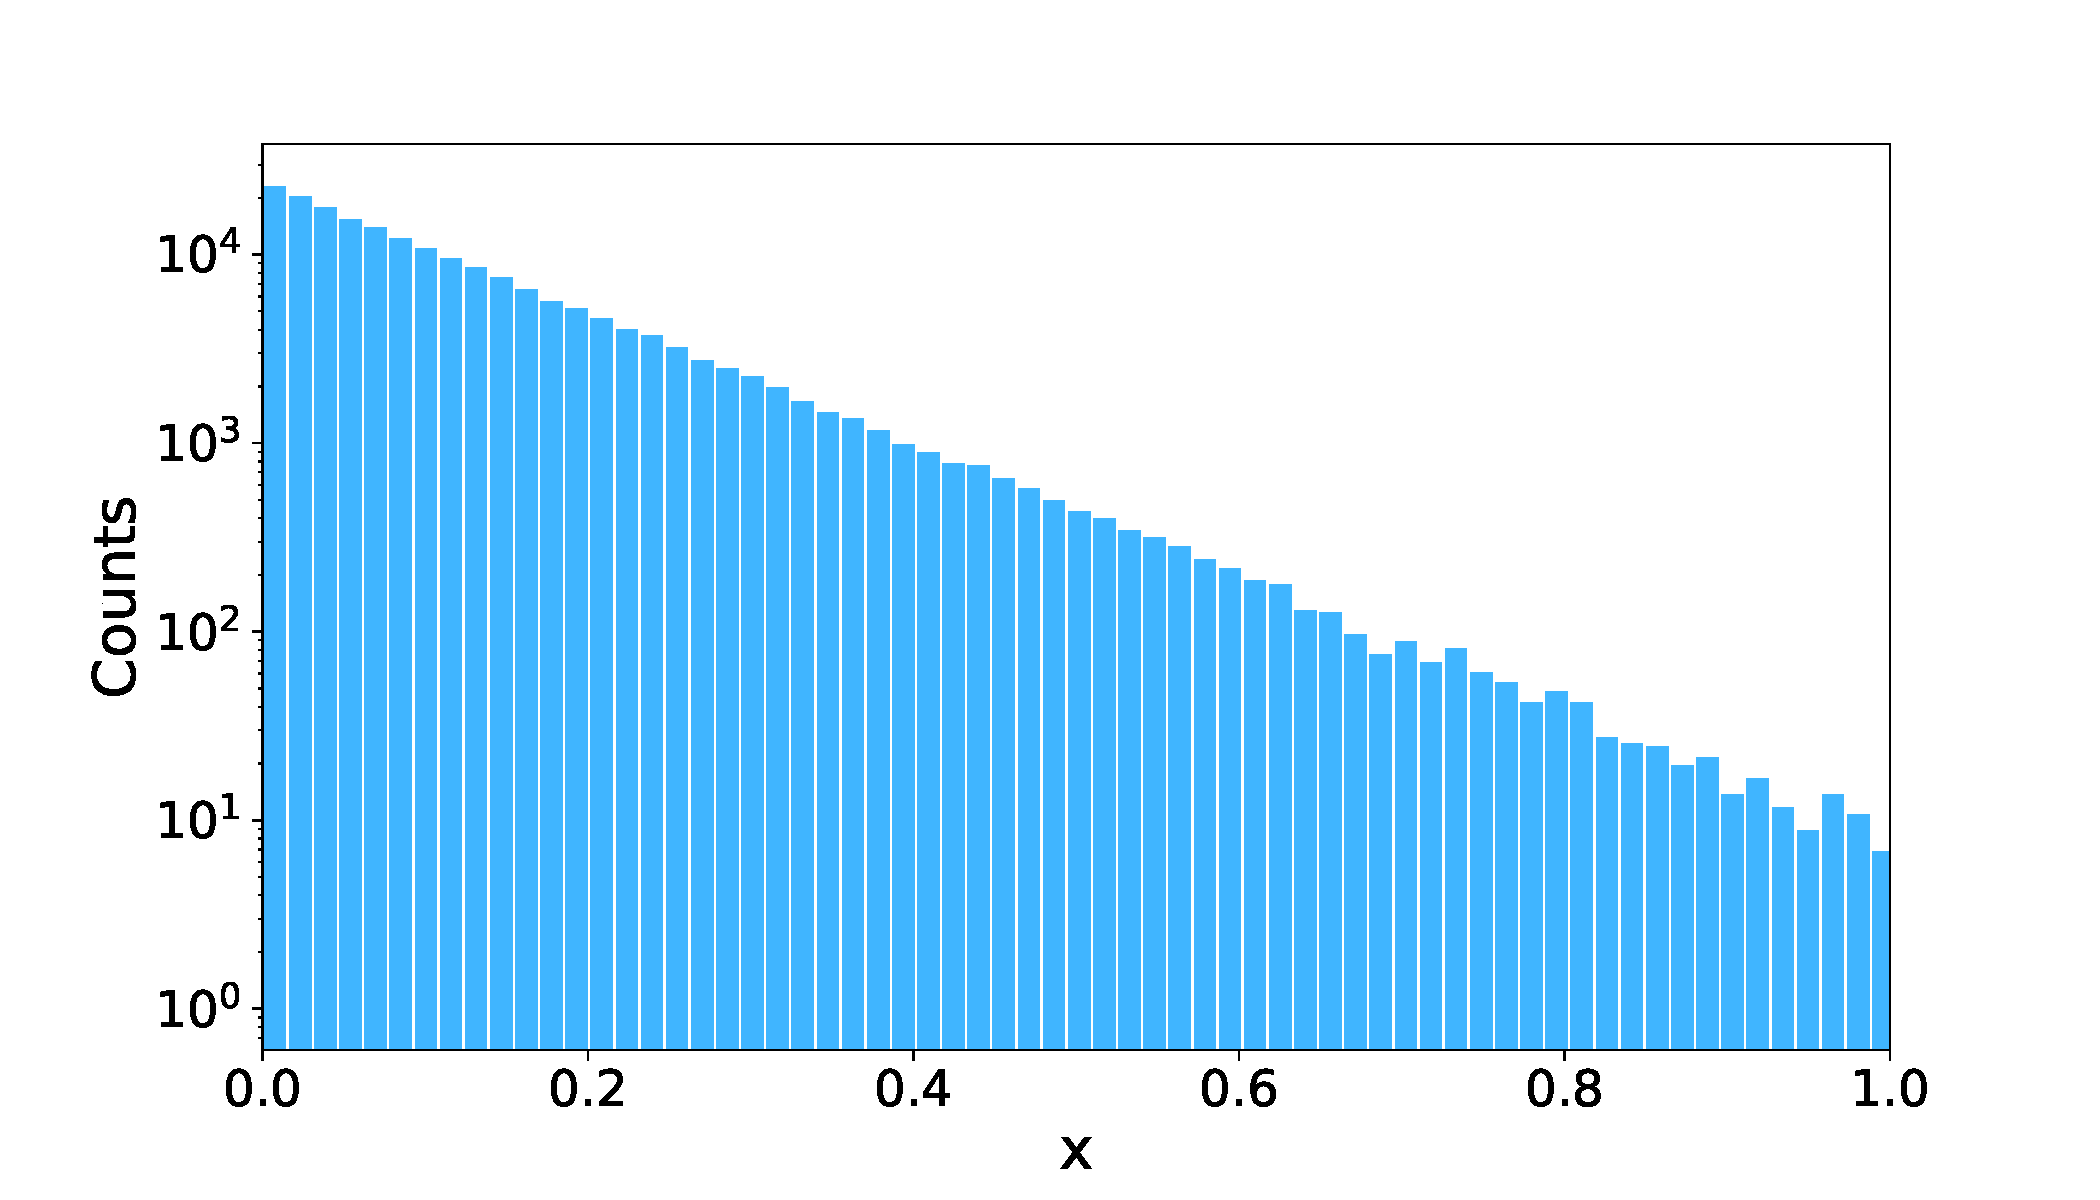
\includegraphics[width=.3\textwidth]{../PLOTS/DISTRIBUTIONS/ref.pdf}};
    \draw[bend left,->, very thick, shorten <=2pt, shorten >=2pt]  (ref) to node [auto] 
    {} (main);


    % LOWER LEFT
    \node(exp)[below left = -1cm and 0cm of main, label={[label distance=-0.4cm]above:\bfseries  data sample $\mathbfcal{D}$}]  
    {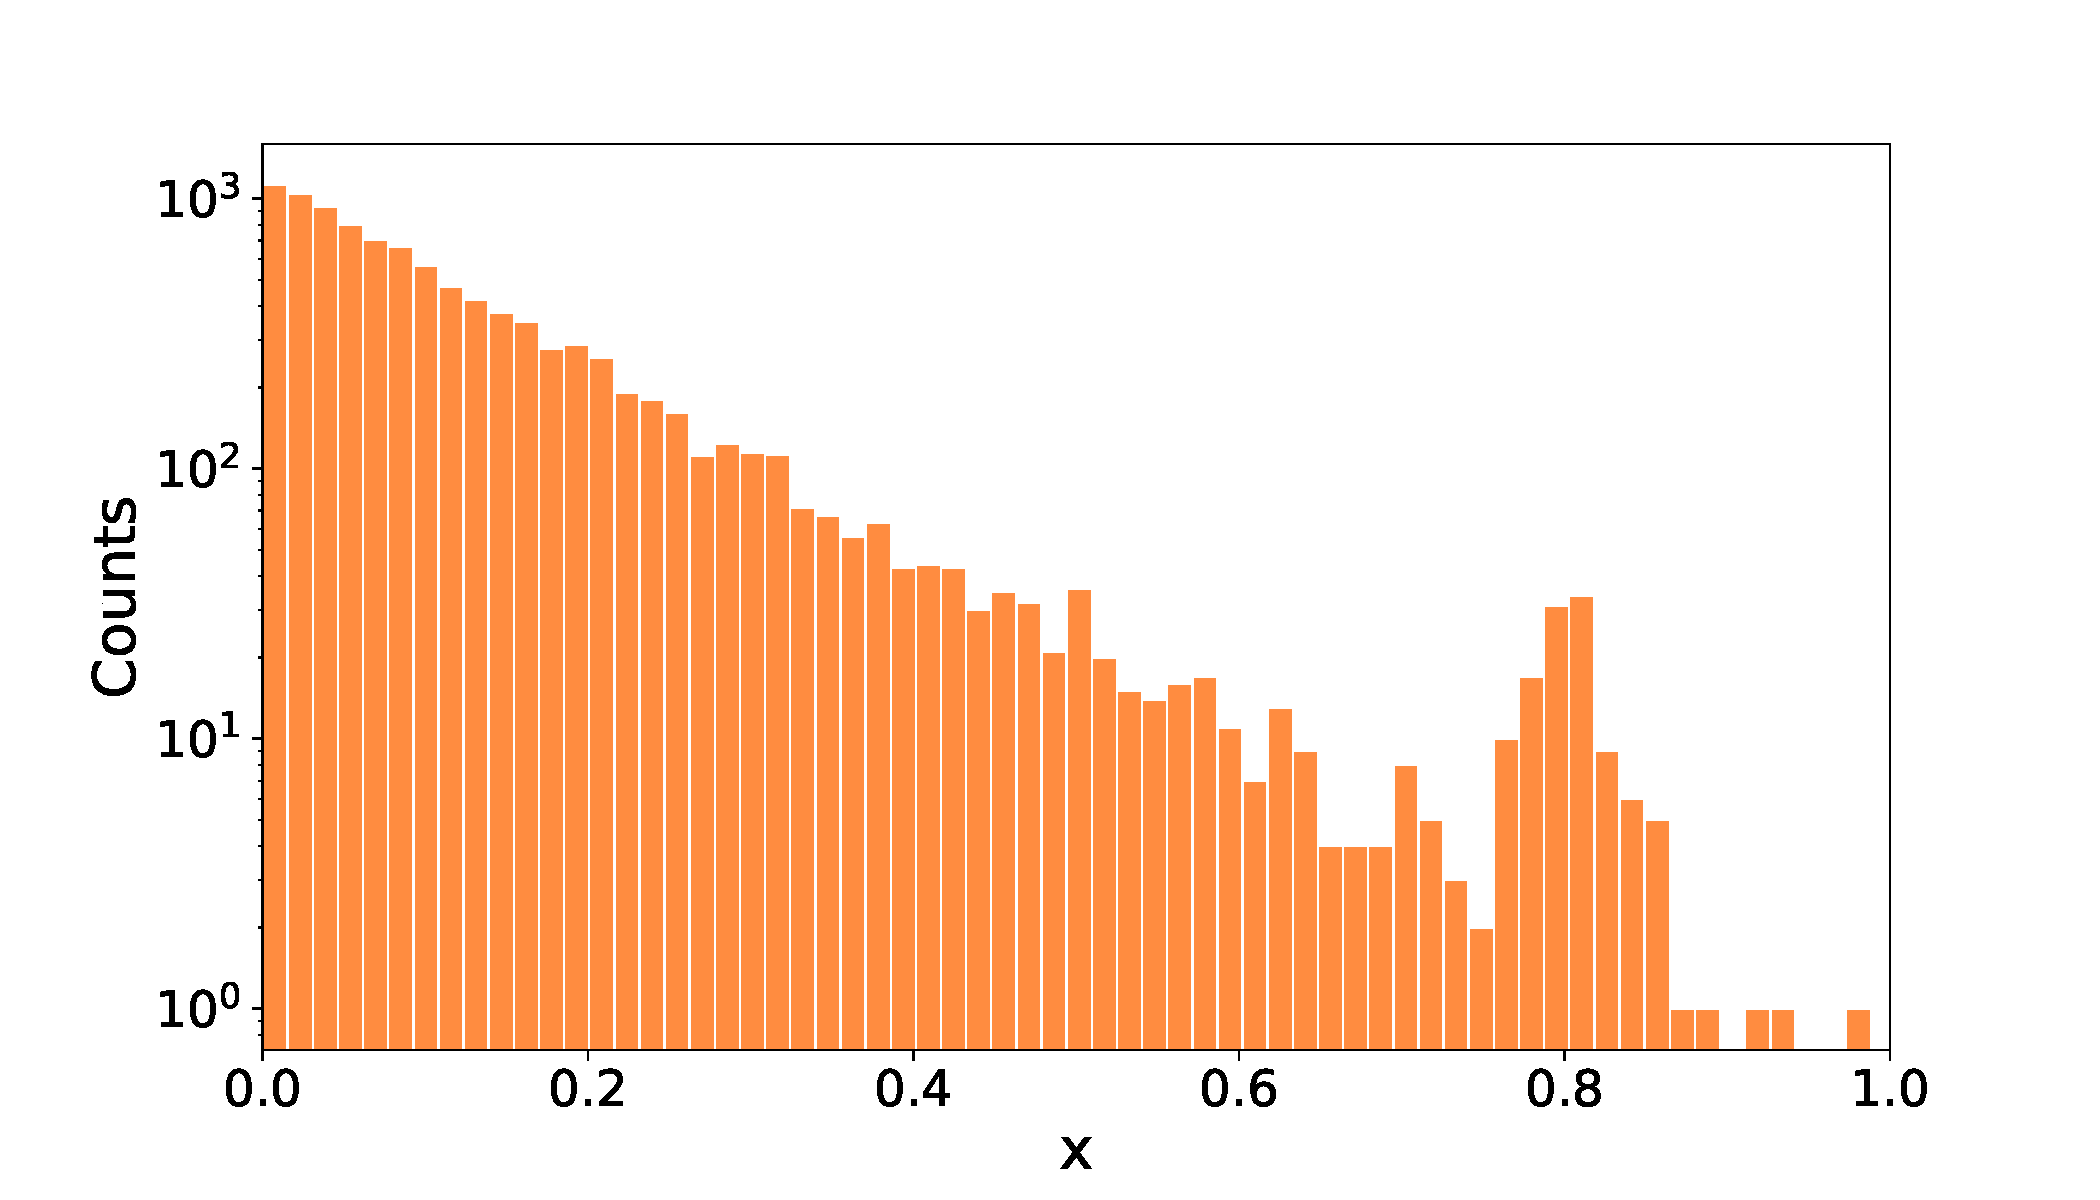
\includegraphics[width=.3\textwidth]{../PLOTS/DISTRIBUTIONS/exp.pdf}};
    \draw[bend right,->, very thick, shorten <=2pt, shorten >=2pt]  (exp) to node [auto] 
    {} (main);

    % UPPER RIGHT
    \node(log)[above right = -1cm and 0cm of main, label={[align=center, label distance=-0.4cm]above:\bfseries  log-ratio distribution \\ 
    $f(x;\,\hat{w})\approx \log\left[\frac{n(x\,|\,\mathbfcal{T})}{n(x\,|\,\mathbfcal{R})}\right]$}] 
    {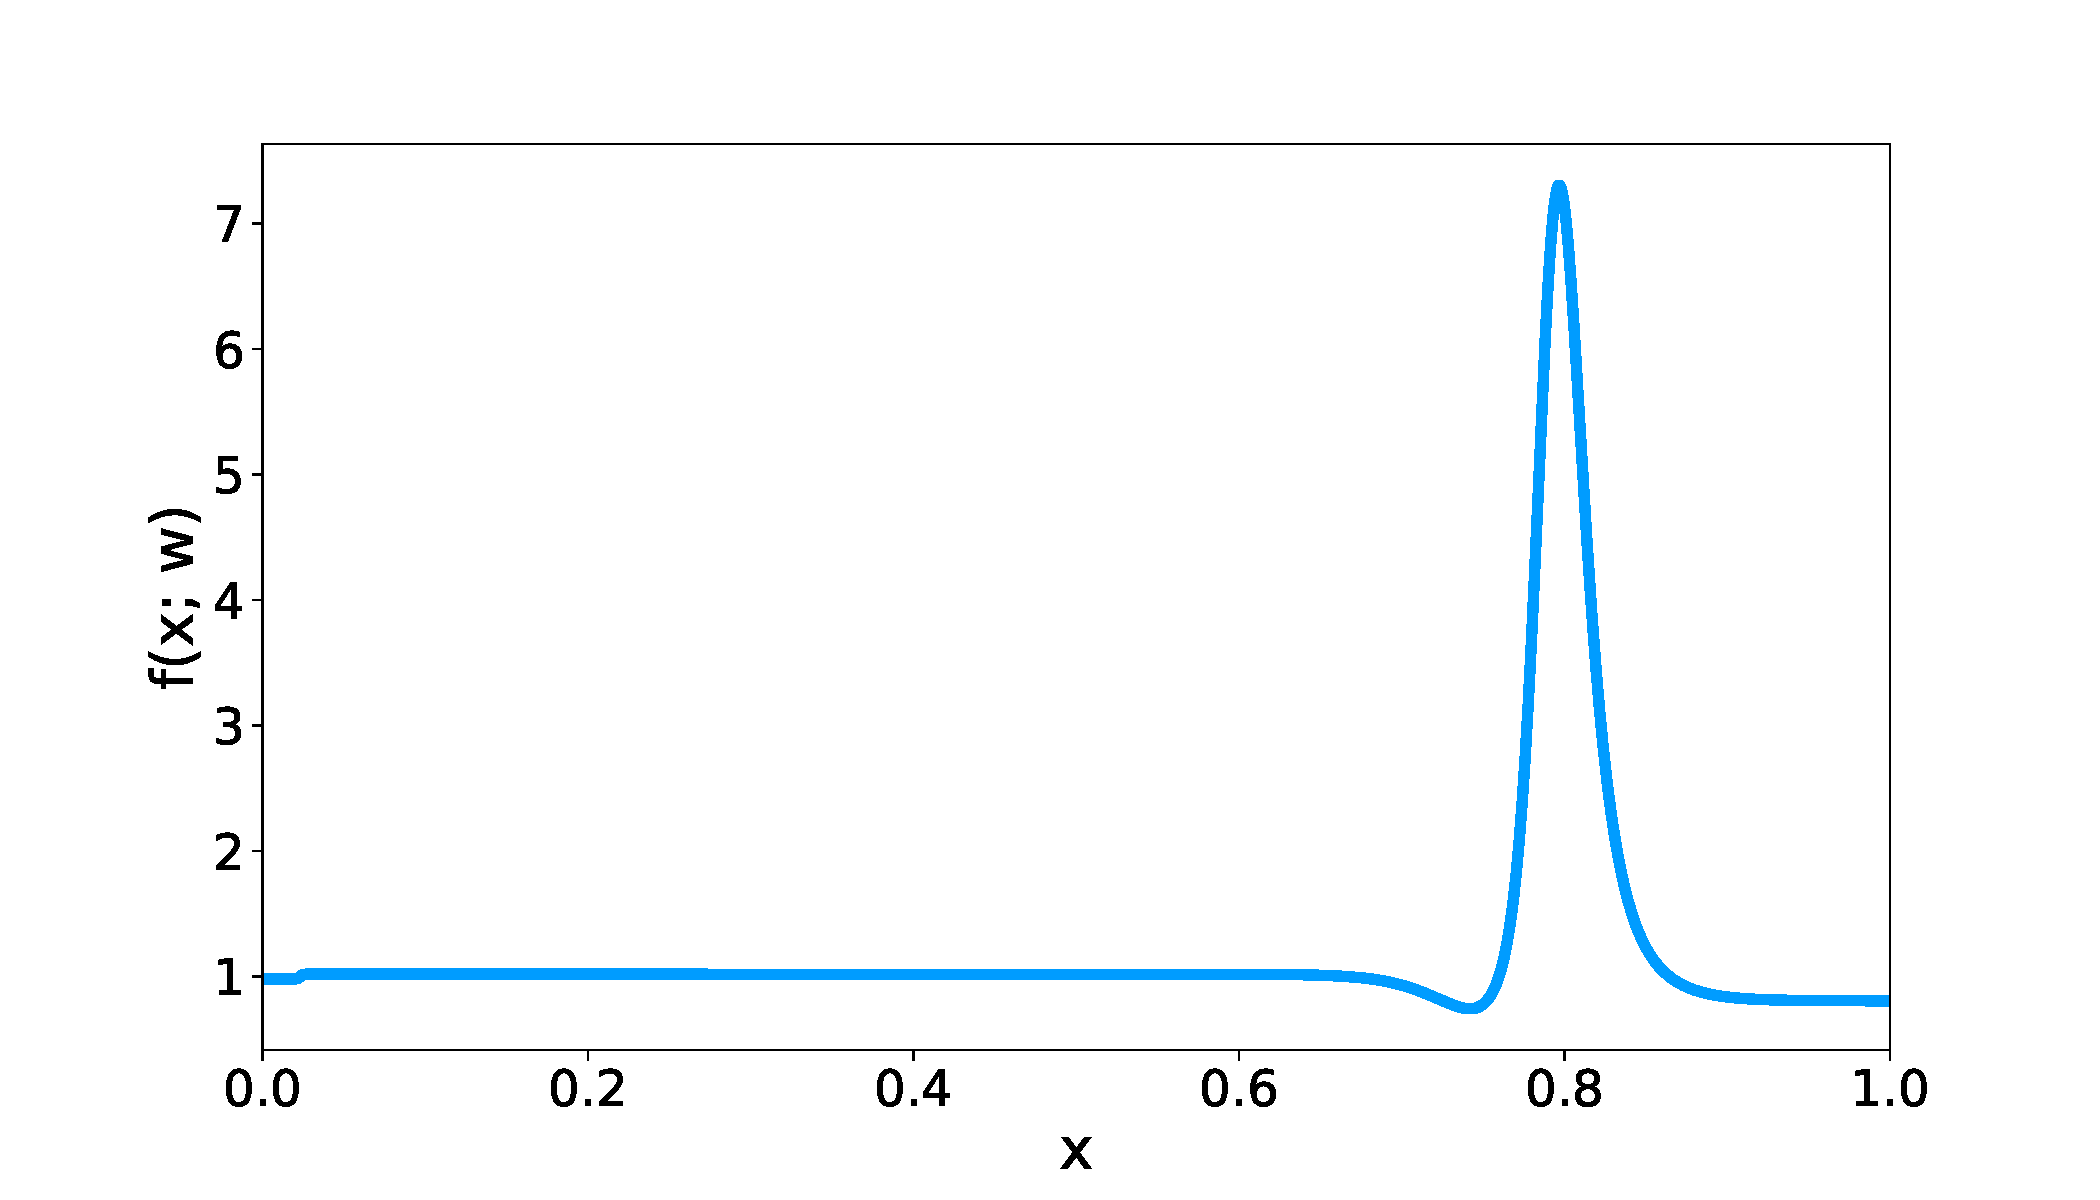
\includegraphics[width=.3\textwidth]{../PLOTS/DISTRIBUTIONS/log_ratio_47.pdf}};
    \draw[bend left,->, very thick, shorten <=2pt, shorten >=2pt]  (main) to node [auto] 
    {} (log);


    % LOWER RIGHT
    \node(t)[below right = -1cm and 0cm of main, label={[align=center, label distance=-0.4cm]above:\bfseries $\boldsymbol{t}$ distribution \\
    $t(\mathbfcal{D})=-2\,\min_w L[f]$}]  
    {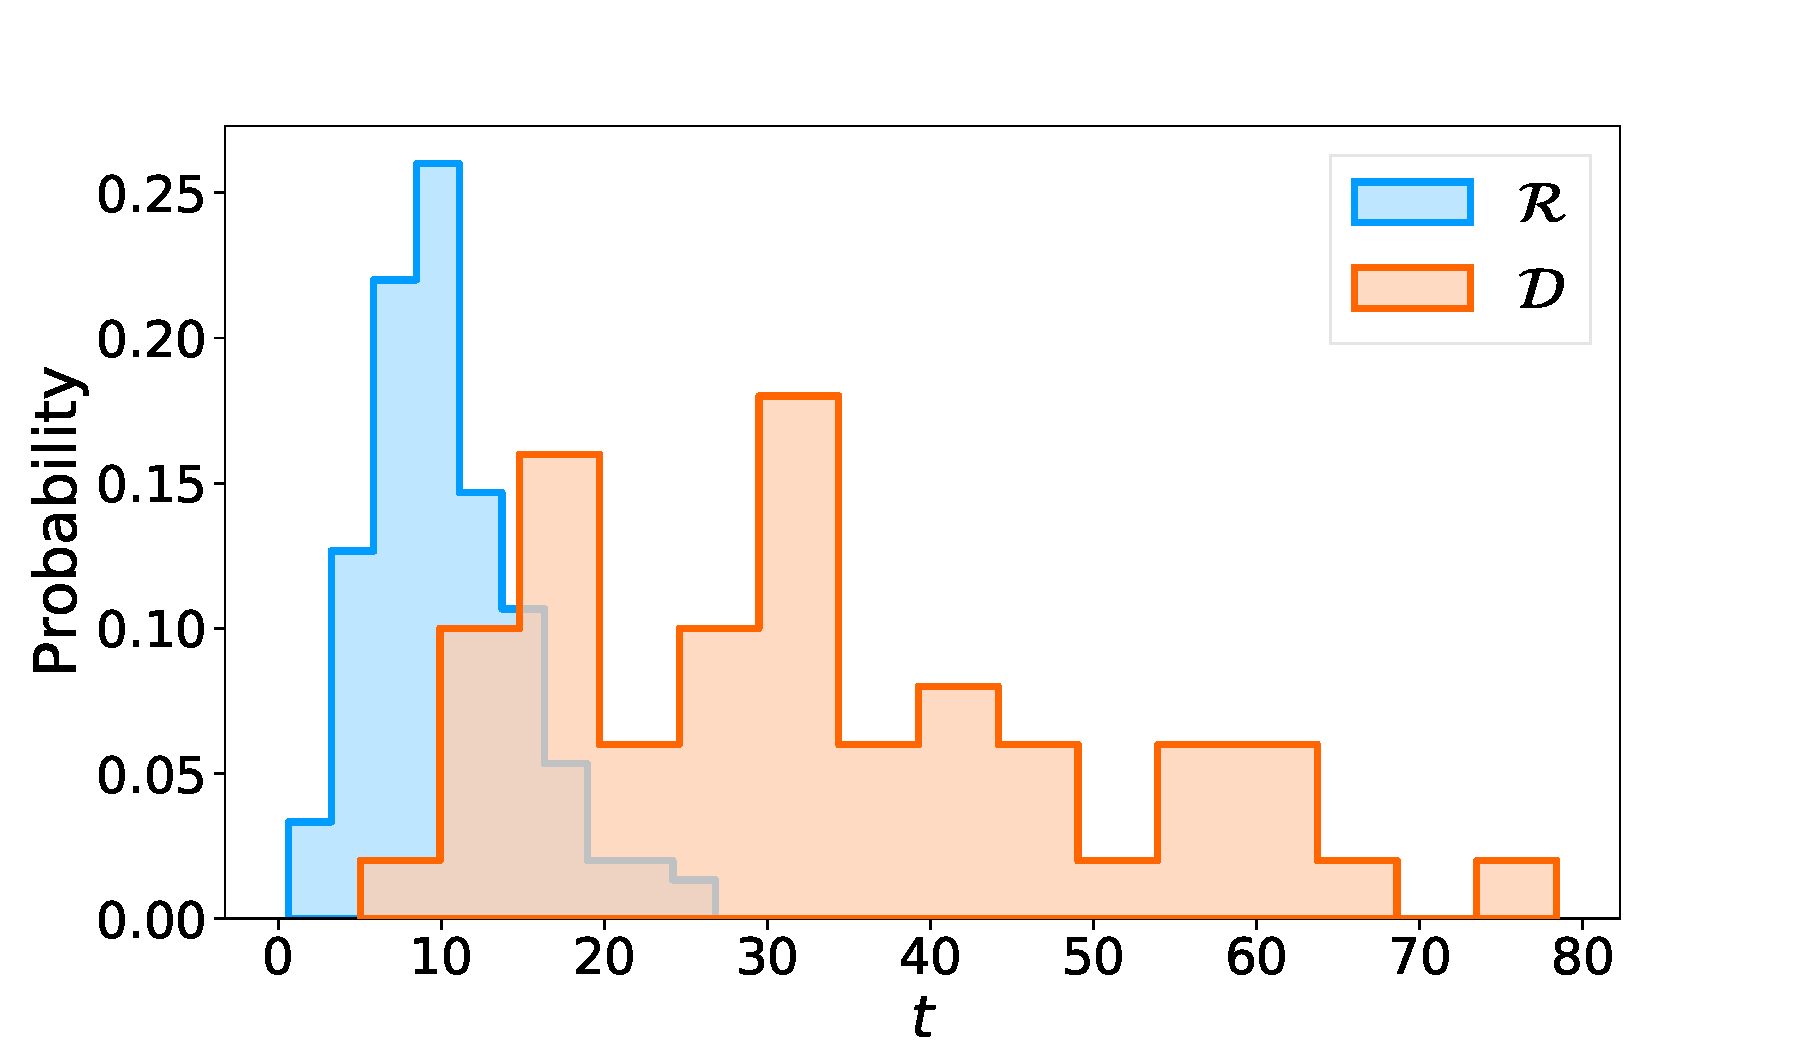
\includegraphics[width=.3\textwidth]{../PLOTS/DISTRIBUTIONS/summary_distribution.pdf}};
    \draw[bend right,->, very thick, shorten <=2pt, shorten >=2pt]  (main) to node [auto] 
    {} (t);

    % INPUT
    \node(in)[above = 1.5cm of ref]{\bfseries INPUT};

    % OUTPUT
    \node(out)[above = 1.5cm of log]{\bfseries OUTPUT};

\end{tikzpicture}}
	\captionof{figure}{Visual representation of the algorithm}
	\label{fig:summary}
\end{figure} 



\section{Technical implementation of the algorithm}

A sufficient amount of toy experiments, sampled from the reference dataset, is necessary to successfully tune the
network hyperparameters. Moreover, a changing yet large amout of training epochs are needed to reach an acceptable
compatibility with the expected $\chi^2_{\nu}$ distribution. Thus, running the algorithm turns out to be computationally
heavy: tasks parallelization is mandatory to achieve the desired results in a reasonable amout of time.  
Then, a cluster of machines, located in Legnaro and Padova, was used and jobs were submitted via Condor. In order to
submit the jobs to the batch system, the t2-ui-12 machine was accessed via ssh tunnel through the infn gate.

The alghorithm has been implemented in Python using the Keras module. The optimizer used to minimize the loss function
is ADAM, as implemented in Keras with the TensorFlow backend, with an initial learning rate set to $10^{-3}$ and
parameters $\beta_1=0.9$, $\beta_2=0.99$, $\epsilon=10^{-7}$. The batch size has been kept fixed to cover the whole
training sample throughout the work. 

\begin{figure}[h]
	\centering
	% Fully Connected Neural Network

\def\layersep{2.5cm}
\resizebox{!}{0.35\paperheight}{%
\begin{tikzpicture}[shorten >=1pt,->,draw=black!50, node distance=\layersep, scale=0.5]
    \tikzstyle{every pin edge}=[<-,shorten <=1pt]
    \tikzstyle{neuron}=[circle,fill=black!25,minimum size=15pt,inner sep=0pt]
    \tikzstyle{input neuron}=[neuron, fill=green!40];
    \tikzstyle{output neuron}=[neuron, fill=red!40];
    \tikzstyle{hidden neuron}=[neuron, fill=blue!40];
    \tikzstyle{annot} = [text width=6em, text centered]

    
    % Draw the hidden layer nodes
    \foreach \name / \y in {1,...,3}
        \path[yshift=0.5cm]
            node[hidden neuron,draw=black!100,thick] (H-\name) at (2*\layersep,-1.4*\y cm) {};

        % Draw the input layer nodes
    \node[input neuron,draw=black!100,thick,pin=left:{\scriptsize input}] (I-1)
    [left=1.25*\layersep of H-2] {};

    % Draw the output layer node
    \node[output neuron,draw=black!100,thick,pin={[pin edge={->}]right:{\scriptsize output}}] (O-1)
    [right=1.25*\layersep of H-2] {};


    % Connect every node in the input layer with every node in the
    % hidden layer.
    \foreach \dest in {1,...,3}
        \path (I-1) edge (H-\dest);

    % Connect every node in the hidden layer with the output layer
    \foreach \source in {1,...,3}
        \path (H-\source) edge (O-1);

    % Annotate the layers
    \node[label={Hidden Layer}, above=0.3cm] (h_l) at (H-1) {};
    \node[label={Input Layer}] (i_l) [left=0cm and 1.6*\layersep of h_l] {};
    \node[label={Output Layer}] (o_l) [right=0cm and 1.6*\layersep of h_l] {};

    % % Annotate the free parameters
    % \node[label={Hidden Layer}, below=1.3cm] (h_w) at (H-3) {};
    % \node[label={Input Layer}] (i_w)  [left=1.25*\layersep of h_w] {};
    % \node[label={Output Layer}] (o_w) [right=1.25*\layersep of h_w] {};

     
    \node[annot,below of=H-1, node distance=2.5cm] (bhl) {\textbf{3} weights\\\textbf{3} biases};
    \node[annot,right of=bhl, node distance= 1.6*\layersep] {\textbf{3} weights\\\textbf{1} bias};

\end{tikzpicture}}
	\captionof{figure}{Architecture of the implemented neural network with explicit counting of free parameters}
	\label{fig:net}
\end{figure}  

The NN architecture that has been chose is quite a simple one: three layers (one input layer, one hidden layer and one
output layer) with the hidden layer having three neurons. The number of degrees of freedom of the network, assumed to be
equal to the number of free parameters, follows

\begin{equation}
    N_{\text{par}}(\vec{a})=\sum_{n=1}^{L-1} a_n \, (a_{n-1} + 1)
\end{equation}

\noindent where $L$ is the number of layers and $a_n$ represents the number of neurons for the $n$-th layer. Thus, for
the NN employed in this work ($1 \times 3 \times 1$) the number of free parameters is $10$. A visual representation of
the NN architecture and an explicit counting of the free parameters is shown in \autoref{fig:net}. 

Regarding activation functions, several have been tested. The internal activation (i.e. the hidden layer activation)
that performed the best is the hyperbolic tangent. The sigmoid activation, although being a valid alternative, makes the
network less elastic and converges slower to the final estimate of $t$. 

Ultimately, the algorithm necessarly requires some sort of regularization, as the loss function (\ref{eq:loss}) is
unbounded from below, meaning that it approaches $-\infty$ if the output of the network diverges for some values of
$x\in\mathbfcal{D}$. The solution that has been implemented is the application of the so-called \textit{weight clipping
W}. In other words, the dangerous possibility for the loss function to reach $-\infty$ is avoided by enforcing an upper
bound on the absolute value of each weight. It has to be stressed that the correct choice of this parameter $W$ is
crucial to get reasonable results: if the constraint is set too tight then the distribution of the test statistic in the
reference hypothesis will turn out to be shifted to the left of the expected $\chi^2_{\nu}$. On the other hand, if the
constraint is set too loose the $t$ distribution will be shifted to the right of $\chi^2_{\nu}$. A detailed discussion
on the procedure adopted to find the right weight clipping, along with some visual examples, can be found in the
following section. 


\section{Behaviour and performance on simulated data}
\label{sec:testdata}

Plots e cose fighe 